\newpage
\chapter{Волна де Бройля. Волновые пакеты}
\par  В 1924 г. французский физик Луи де Бройль выдвинул смелую гипотезу, согласно которой корпускулярно-волновой дуализм имеет универсальный характер. Согласно его гипотезе каждая материальная частица обладает волновыми свойствами, причем соотношения, связывающие волновые и корпускулярные характеристики частицы остаются такими же, как и в случае электромагнитного излучения: \textit{"у каждой частицы есть некое поле, зависящее от $\vec{r}$, описывающее её, тогда можем это поле проквантовать (дискретизировать)"}. Т.е. с каждой частицей связана некая плоская волна какого-то комплексного поля $ \psi (\vec{r}, t) =\psi _0 e^{i \vec{k} \vec{r} - i w t} $.
\par Возникает вопрос, что это за неизвестная функция и как она связана с движением частицы. Чисто эмпирически были выявлены следующие соотношения, связывающие волновые и корпускулярные свойства частицы: $\vec{p} = \hbar \vec{k}$, $E= \hbar w$ (*). Вычислим фазовую скорость, т.е. скорость, с которой распространяются точки волны с постоянной фазой:
$$ v_ф = \frac{w}{k} = \frac{E}{p} = \frac{p^2}{2mp}= \frac{v}{2} $$
\par Вот и 1 неприятность: можем отказаться от уравнений Ньютона, понятия траектории и постулировать, что скорость частицы как раз \textit{v}, но это неправильно, ведь тогда придется отказаться от постулатов (*). Как быть? Во-первых, выражение для некой $ \psi (\vec{r}, t) $ патологично, ведь эта функция делокализована в пространстве полностью. Пока мы толком не знаем, что такое электрон, но по неведомым причинам в классической механике это то, что считается шариком, распространено во всем пространстве и по модулю в квадрате описывается функцией, которая сюда войти не может, что не исключено, но странно (??? Не понятно, что он вообще имел в виду).  Из соображения разумности хочется иметь описание, которое иногда приходило бы в движение шарика по орбите, иногда совершало бы какие-то чудеса (например, описывающее строение атома или еще что-нибудь), но эта функция не содержит ни намека на хороший переход к классике, т.е. не удовлетворяет ГУ. Как тогда с помощью $\psi$ проэмитировать движение частицы? Исправить ситуацию может собрание \textit{волнового пакета} - совокупности волн с разными импульсами (много фурье-гармоник), которую описывает волновая функция, заметно отличная от нуля только в очень малом участке пространства, размеры которого можно стремить к нулю вместе с $\hbar$. Если проинтегрировать в k-пространстве $\int_{k- \Delta k}^{k+ \Delta k} e^{ikx} dk = \frac{sin x}{x}$, а в реальном пространстве эта функция локализована. Рассматривая совокупность плоских волн с близкими k в каком-то интервале, соберем пространственный импульс, получим некоторую область, где $\psi$-функция в реальном пространстве не равна нулю в какой-то области, так же требуем, чтоб центр волнового пакета перемещался по истинной траектории классической частицы. Пробуем для простоты в 1D случае:
$$ \psi (x, t) = \int_{- \infty}^{\infty} с(p)  \psi _0 e^{\frac{i(px-E(p)t}{\hbar}} dp $$
\par Нормировка: $$\int | \psi |^2 dx = \iint dp \, dp^\prime c(p)c(p^\prime) | \psi _0 |^2 e^{\frac{i(E\prime-E)t}{\hbar}}  \underbrace{\int e^{\frac{i(p-p^\prime)x}{\hbar}} dx}_{\text{а это } 2 \pi \hbar \delta (p-p^\prime)}=  2 \pi \hbar  | \psi _0 |^2 \int |c|^2 dp $$
\par 
\begin{wrapfigure}[11]{r}{0.3\linewidth} 
\vspace{-2ex}
\centering
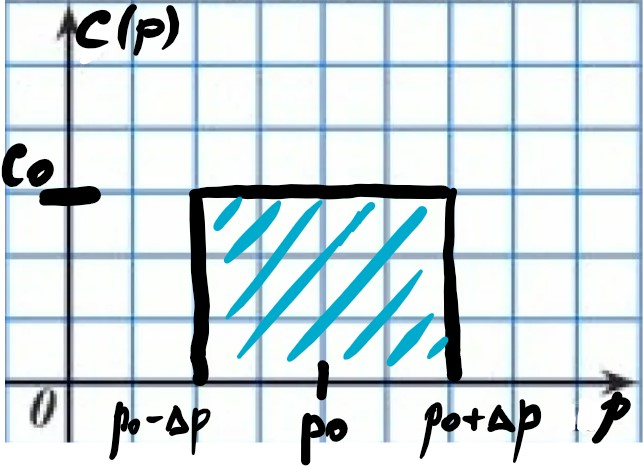
\includegraphics[width=0.8\linewidth]{pictures/4.1.jpg}
\caption{Выбор константы}
\end{wrapfigure}
\par Подберем
$ \psi _0 =\frac{1}{\sqrt{2 \pi \hbar}} $, дальше, если подобрать правильное поводение \textit{с} на $\infty$, можем обеспечить регулярный характер поведения этой нормы. Предположим, что зависимость такая: $c_0 = 1, p \in (p_0- \Delta p, p_0 + \Delta p ) $. Раскладываем вблизи $p_0$ энергию и ищем волновую функцию:
$$ E(p)= E_0 + (p-p_0) \frac{dE}{dp} \bigg|_{p=p_0} $$
$$ \psi = c_0 \int_{p_o - \Delta p}^{p_o + \Delta p} \frac{1}{\sqrt{2 \pi \hbar}} e^{\frac{i(px-Et)}{\hbar}} dp =\bigg| p=p_0+ \hbar \xi \bigg| =\frac{c_0 \hbar}{\sqrt{2 \pi \hbar}} e^{\frac{i(p_0x-E_0t)}{\hbar}} \int_{\frac{ - \Delta p}{\hbar}}^{\frac{ \Delta p}{\hbar}} \,e^{i \xi (x- \frac{dE}{dp})|_{p=p_0} t } \, d \xi =$$
$$=\frac{c_0 \hbar}{\sqrt{2 \pi \hbar}} e^{\frac{i(p_0x-E_0t)}{\hbar}} \cdot 2 \frac{sin(\Delta p) (x- \frac{dE}{dp}|_{p=p_0} t )}{\hbar (x- \frac{dE}{dp}|_{p=p_0} t )} $$
\par Получилась функция $\frac{sin(\frac{\Delta p \chi}{\hbar})}{\chi}$, которая локализована вблизи $\Chi = 0$, т.е. центра масс пакета движется с групповой скоростью (максимум функции при любых временах лежит в одной точке) $x=\frac{dE}{dp}|_{p=p_0} t = \frac{p_0 t}{m} = v_0 t $ равномерно, что не противоречит II закону Ньютона ($ \dot{v} =0$) в отсутствии действия внешней силы). Что отсюда важного стоит извлечь: у этого пакета есть ширина, а сама функция отлична от нуля, когда ее аргумент </порядка 1: $ \frac{\Delta p \cdot \Delta x}{\hbar} \sim 1 $. Т.е. пакет движется примерно по классической траектории частицы, но при этом точность определения ее зависит от точности определения импульса: при размывании $\Delta p$ размывается и $\Delta x$. Возникает соотношение неопределенности $ \Delta p \cdot \Delta x \sim 2 \pi h $
\par Энергия связана с импульсом, мы предполагали, что $E \sim e^{-iwt} $, а значит, если посчитать то же самое при $p^2 $, пакет "расплывётся".
 